% Options for packages loaded elsewhere
\PassOptionsToPackage{unicode}{hyperref}
\PassOptionsToPackage{hyphens}{url}
%
\documentclass[
  man,floatsintext]{apa6}
\usepackage{amsmath,amssymb}
\usepackage{lmodern}
\usepackage{iftex}
\ifPDFTeX
  \usepackage[T1]{fontenc}
  \usepackage[utf8]{inputenc}
  \usepackage{textcomp} % provide euro and other symbols
\else % if luatex or xetex
  \usepackage{unicode-math}
  \defaultfontfeatures{Scale=MatchLowercase}
  \defaultfontfeatures[\rmfamily]{Ligatures=TeX,Scale=1}
\fi
% Use upquote if available, for straight quotes in verbatim environments
\IfFileExists{upquote.sty}{\usepackage{upquote}}{}
\IfFileExists{microtype.sty}{% use microtype if available
  \usepackage[]{microtype}
  \UseMicrotypeSet[protrusion]{basicmath} % disable protrusion for tt fonts
}{}
\makeatletter
\@ifundefined{KOMAClassName}{% if non-KOMA class
  \IfFileExists{parskip.sty}{%
    \usepackage{parskip}
  }{% else
    \setlength{\parindent}{0pt}
    \setlength{\parskip}{6pt plus 2pt minus 1pt}}
}{% if KOMA class
  \KOMAoptions{parskip=half}}
\makeatother
\usepackage{xcolor}
\IfFileExists{xurl.sty}{\usepackage{xurl}}{} % add URL line breaks if available
\IfFileExists{bookmark.sty}{\usepackage{bookmark}}{\usepackage{hyperref}}
\hypersetup{
  pdftitle={Satisfying housework division? Gender role beliefs and religion as moderators of housework division and satisfaction},
  pdfauthor={Carlotta Reinhardt1, Margaret Bassney1, \& Anushree Goswami1},
  pdflang={en-EN},
  hidelinks,
  pdfcreator={LaTeX via pandoc}}
\urlstyle{same} % disable monospaced font for URLs
\usepackage{graphicx}
\makeatletter
\def\maxwidth{\ifdim\Gin@nat@width>\linewidth\linewidth\else\Gin@nat@width\fi}
\def\maxheight{\ifdim\Gin@nat@height>\textheight\textheight\else\Gin@nat@height\fi}
\makeatother
% Scale images if necessary, so that they will not overflow the page
% margins by default, and it is still possible to overwrite the defaults
% using explicit options in \includegraphics[width, height, ...]{}
\setkeys{Gin}{width=\maxwidth,height=\maxheight,keepaspectratio}
% Set default figure placement to htbp
\makeatletter
\def\fps@figure{htbp}
\makeatother
\setlength{\emergencystretch}{3em} % prevent overfull lines
\providecommand{\tightlist}{%
  \setlength{\itemsep}{0pt}\setlength{\parskip}{0pt}}
\setcounter{secnumdepth}{-\maxdimen} % remove section numbering
% Make \paragraph and \subparagraph free-standing
\ifx\paragraph\undefined\else
  \let\oldparagraph\paragraph
  \renewcommand{\paragraph}[1]{\oldparagraph{#1}\mbox{}}
\fi
\ifx\subparagraph\undefined\else
  \let\oldsubparagraph\subparagraph
  \renewcommand{\subparagraph}[1]{\oldsubparagraph{#1}\mbox{}}
\fi
\newlength{\cslhangindent}
\setlength{\cslhangindent}{1.5em}
\newlength{\csllabelwidth}
\setlength{\csllabelwidth}{3em}
\newlength{\cslentryspacingunit} % times entry-spacing
\setlength{\cslentryspacingunit}{\parskip}
\newenvironment{CSLReferences}[2] % #1 hanging-ident, #2 entry spacing
 {% don't indent paragraphs
  \setlength{\parindent}{0pt}
  % turn on hanging indent if param 1 is 1
  \ifodd #1
  \let\oldpar\par
  \def\par{\hangindent=\cslhangindent\oldpar}
  \fi
  % set entry spacing
  \setlength{\parskip}{#2\cslentryspacingunit}
 }%
 {}
\usepackage{calc}
\newcommand{\CSLBlock}[1]{#1\hfill\break}
\newcommand{\CSLLeftMargin}[1]{\parbox[t]{\csllabelwidth}{#1}}
\newcommand{\CSLRightInline}[1]{\parbox[t]{\linewidth - \csllabelwidth}{#1}\break}
\newcommand{\CSLIndent}[1]{\hspace{\cslhangindent}#1}
\ifLuaTeX
\usepackage[bidi=basic]{babel}
\else
\usepackage[bidi=default]{babel}
\fi
\babelprovide[main,import]{english}
% get rid of language-specific shorthands (see #6817):
\let\LanguageShortHands\languageshorthands
\def\languageshorthands#1{}
% Manuscript styling
\usepackage{upgreek}
\captionsetup{font=singlespacing,justification=justified}

% Table formatting
\usepackage{longtable}
\usepackage{lscape}
% \usepackage[counterclockwise]{rotating}   % Landscape page setup for large tables
\usepackage{multirow}		% Table styling
\usepackage{tabularx}		% Control Column width
\usepackage[flushleft]{threeparttable}	% Allows for three part tables with a specified notes section
\usepackage{threeparttablex}            % Lets threeparttable work with longtable

% Create new environments so endfloat can handle them
% \newenvironment{ltable}
%   {\begin{landscape}\centering\begin{threeparttable}}
%   {\end{threeparttable}\end{landscape}}
\newenvironment{lltable}{\begin{landscape}\centering\begin{ThreePartTable}}{\end{ThreePartTable}\end{landscape}}

% Enables adjusting longtable caption width to table width
% Solution found at http://golatex.de/longtable-mit-caption-so-breit-wie-die-tabelle-t15767.html
\makeatletter
\newcommand\LastLTentrywidth{1em}
\newlength\longtablewidth
\setlength{\longtablewidth}{1in}
\newcommand{\getlongtablewidth}{\begingroup \ifcsname LT@\roman{LT@tables}\endcsname \global\longtablewidth=0pt \renewcommand{\LT@entry}[2]{\global\advance\longtablewidth by ##2\relax\gdef\LastLTentrywidth{##2}}\@nameuse{LT@\roman{LT@tables}} \fi \endgroup}

% \setlength{\parindent}{0.5in}
% \setlength{\parskip}{0pt plus 0pt minus 0pt}

% Overwrite redefinition of paragraph and subparagraph by the default LaTeX template
% See https://github.com/crsh/papaja/issues/292
\makeatletter
\renewcommand{\paragraph}{\@startsection{paragraph}{4}{\parindent}%
  {0\baselineskip \@plus 0.2ex \@minus 0.2ex}%
  {-1em}%
  {\normalfont\normalsize\bfseries\itshape\typesectitle}}

\renewcommand{\subparagraph}[1]{\@startsection{subparagraph}{5}{1em}%
  {0\baselineskip \@plus 0.2ex \@minus 0.2ex}%
  {-\z@\relax}%
  {\normalfont\normalsize\itshape\hspace{\parindent}{#1}\textit{\addperi}}{\relax}}
\makeatother

% \usepackage{etoolbox}
\makeatletter
\patchcmd{\HyOrg@maketitle}
  {\section{\normalfont\normalsize\abstractname}}
  {\section*{\normalfont\normalsize\abstractname}}
  {}{\typeout{Failed to patch abstract.}}
\patchcmd{\HyOrg@maketitle}
  {\section{\protect\normalfont{\@title}}}
  {\section*{\protect\normalfont{\@title}}}
  {}{\typeout{Failed to patch title.}}
\makeatother

\usepackage{xpatch}
\makeatletter
\xapptocmd\appendix
  {\xapptocmd\section
    {\addcontentsline{toc}{section}{\appendixname\ifoneappendix\else~\theappendix\fi\\: #1}}
    {}{\InnerPatchFailed}%
  }
{}{\PatchFailed}
\usepackage{lineno}

\linenumbers
\usepackage{csquotes}
\usepackage[titles]{tocloft}
\cftpagenumbersoff{figure}
\renewcommand{\cftfigpresnum}{\itshape\figurename\enspace}
\renewcommand{\cftfigaftersnum}{.\space}
\setlength{\cftfigindent}{0pt}
\setlength{\cftafterloftitleskip}{0pt}
\settowidth{\cftfignumwidth}{Figure 10.\qquad}
\cftpagenumbersoff{table}
\renewcommand{\cfttabpresnum}{\itshape\tablename\enspace}
\renewcommand{\cfttabaftersnum}{.\space}
\setlength{\cfttabindent}{0pt}
\setlength{\cftafterloftitleskip}{0pt}
\settowidth{\cfttabnumwidth}{Table 10.\qquad}
\ifLuaTeX
  \usepackage{selnolig}  % disable illegal ligatures
\fi

\title{Satisfying housework division? Gender role beliefs and religion as moderators of housework division and satisfaction}
\author{Carlotta Reinhardt\textsuperscript{1}, Margaret Bassney\textsuperscript{1}, \& Anushree Goswami\textsuperscript{1}}
\date{}


\shorttitle{gender roles, housework and satisfaction}

\affiliation{\vspace{0.5cm}\textsuperscript{1} Smith College}

\begin{document}
\maketitle

\hypertarget{results}{%
\section{Results}\label{results}}

\hypertarget{analysis-strategy}{%
\subsection{Analysis Strategy}\label{analysis-strategy}}

To test our hypotheses that gender role beliefs and religion moderate the relationship between housework distribution and satisfaction, we used multilevel modeling and the Actor-Partner Interdependence Model (APIM; THIS NEEDS TO BE A REAL CITATION SO THERE IS A BIBLIOGRAPHY Kenny, Kashy, and Cook (2020)). The APIM measures the effect of the explanatory variables for both members in a dyad at the same time, so actor as well as partner effects could be considered in our analysis. This way, it is possible to see how one partner's housework distribution affects both their own satisfaction with the housework distribution (actor effect) and their partner's satisfaction with the housework distribution (partner effect). In this analysis, we will look at the moderating effect of each partner's gender role beliefs on the two actor effects (shown in figure 1) as well as on the partner effects. (THIS FOLLOWING SENTENCE CONFUSES ME!) Our research studied people in relationships, where each pair in a relationship is refered to as a dyad. Since we were working with dyadic data, our data was not independent. For example the amount of housework one partner does, will be correlated with how much housework the other partner does.This will result in correlated residuals. To account for the nonindependence, the APIM considered how much of the variation in satisfaction was caused by the dyad compared to housework distribution and gender role beleifs. To account for the correlated errors, we weighted each dyad so that the residuals of each individual were constant. (IS THIS BETTER OR WORSE LOL)



\begin{figure}
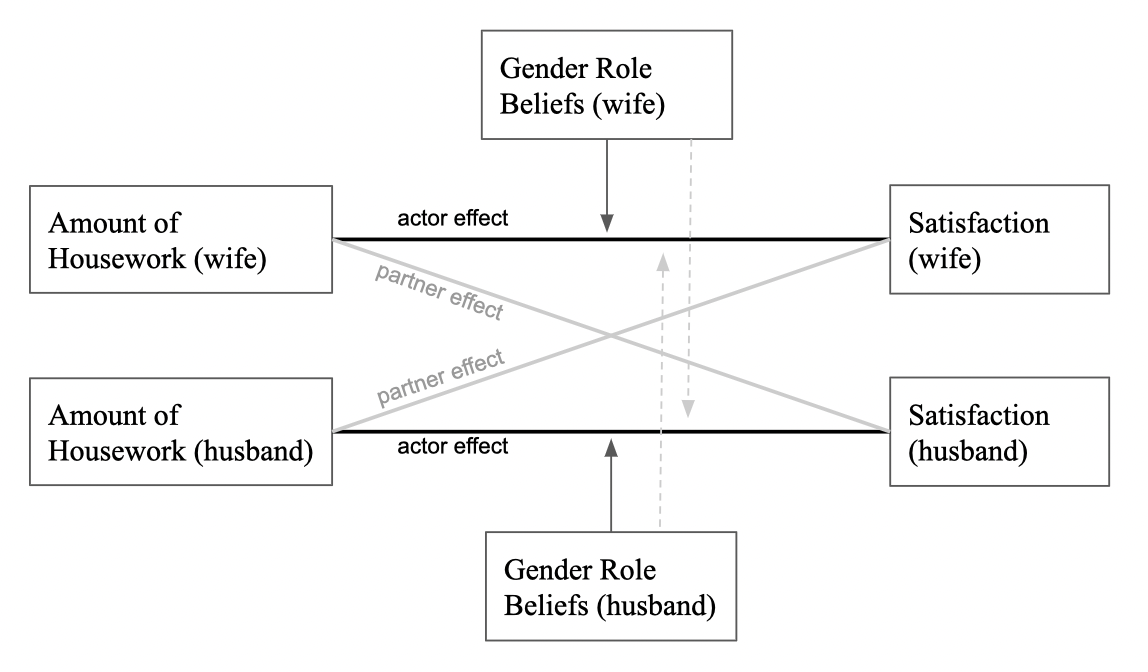
\includegraphics[width=3.83in]{APIM} \caption{Schematic representation of actor and partner effects in the APIM moderated by gender role beliefs.}\label{fig:unnamed-chunk-3}
\end{figure}

\hypertarget{main-results}{%
\subsection{Main Results}\label{main-results}}

\hypertarget{gender-role-beliefs-as-a-moderator}{%
\paragraph{Gender Role Beliefs as a moderator}\label{gender-role-beliefs-as-a-moderator}}

All relevant results of the moderation analysis in the APIM are shown in figure 2. It was shown that for husbands and wives, a higher amount of housework was significantly related to a lower satisfaction (\(\beta\) =-0.02, \emph{p} = 0.02,\(\beta\) =-0.03, \emph{p} = 0.01).
For the female partners, gender role beliefs significantly moderated the relationship between the wives' housework distribution and satisfaction with the housework distribution. The moderation effect was 0.07 (\emph{p} = \textless0.01, SE = 0.02). Higher gender role beliefs, which means more conservative, was therefore associated with a higher satisfaction when the amount of housework was kept constant. The wife's gender role beliefs and husband's gender role beliefs significantly moderated the relationship between the wife's housework distribution and the wife's satisfaction with the housework distribution. The moderation effect was -0.06 (\emph{p} = 0.01, SE = 0.02). When the husbands had more conservative gender role beliefs, the wife's satisfaction decreased by -0.06 while keeping housework distribution constant.
Moreover, a moderation effect was found for the relationship between the husbands amount of housework and the wife's satisfaction which was moderated by the husband's gender role beliefs(\(\beta\) = -0.01, \emph{p} =0.68) . More conservative gender role beliefs were associated with lower satisfaction when housework distribution was held constant 0.07 (INCLUDE NUMBERS).
All other paths were not significantly related to each other (INCLUDE LOWEST OF ALL NONSIGN. P VALUES HERE, AND THEN \emph{p} \textgreater{} \ldots)



\begin{figure}
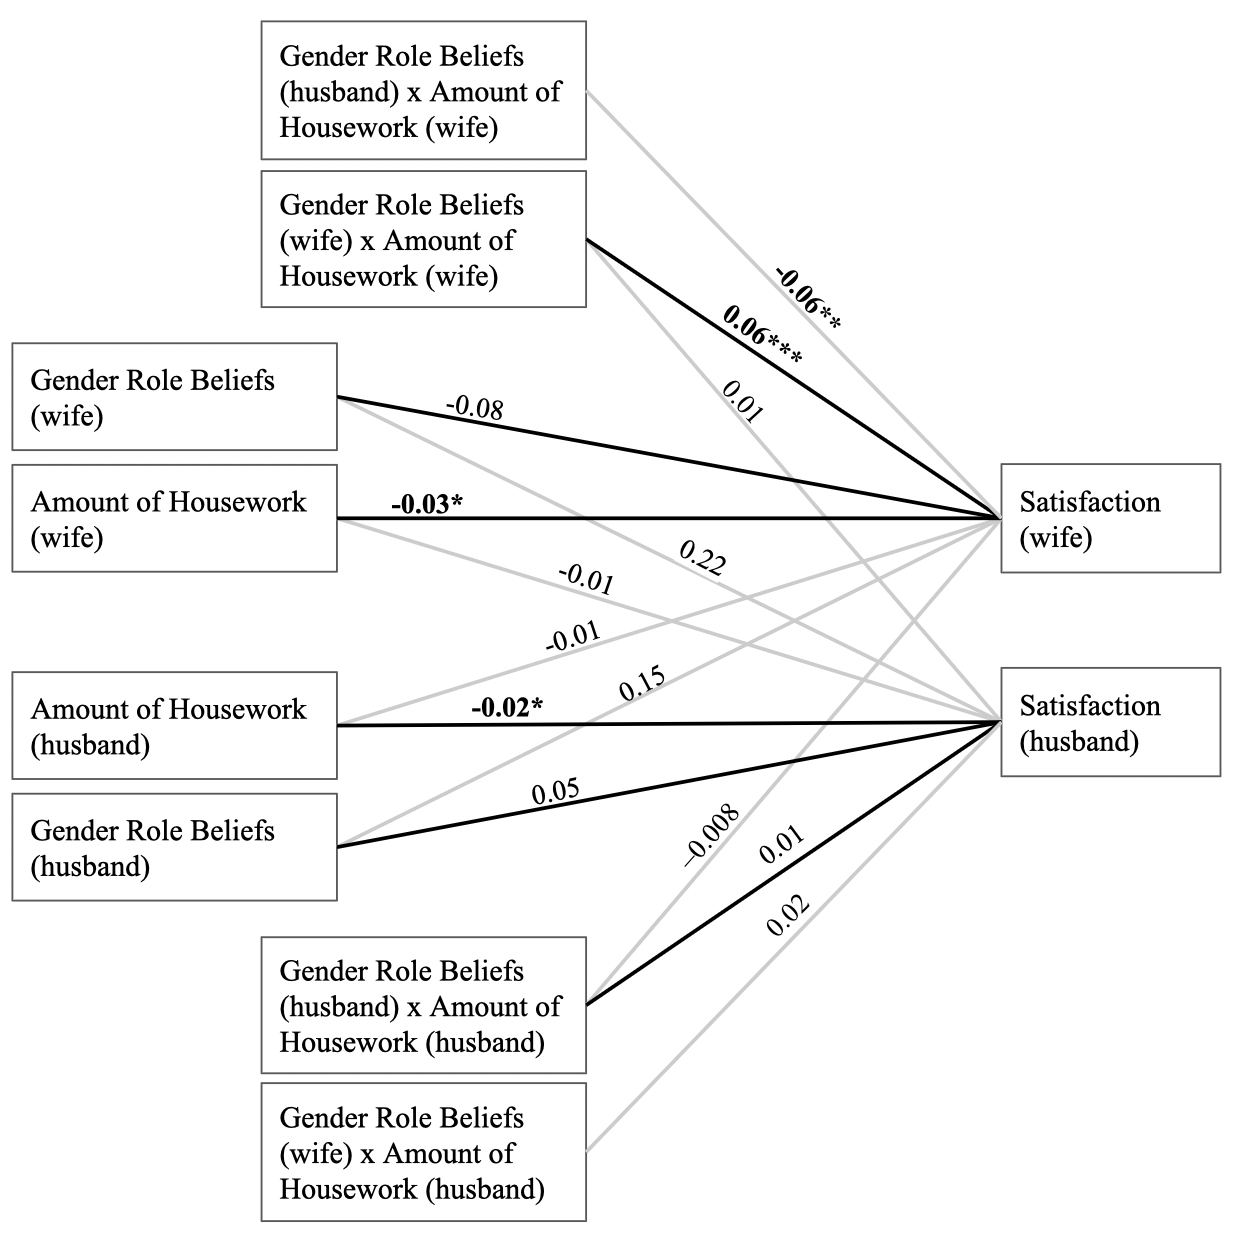
\includegraphics[width=4.25in]{moderation} \caption{Moderation effects in the APIM. Values shown in the figure are uncorrected b coefficients (PLEASE TRY TO FIND WHAT THE NUMBERS MEAN, I AM LOST - i dont understand what you mean by uncorrected b coefficients).}\label{fig:unnamed-chunk-9}
\end{figure}

(I DON'T UNDERSTAND THIS SENTENCE/SECTION. WHAT IS DESCRIBED HERE? THAT MUST BE CLEAR AND RELATED TO A FIGURE ETC.)(By design gender is a moderator, so explaining gender differences) Only looking at the three way interactions with gender we found two significant gender differences in the moderation effects. The interaction between actors housework distribution and their own gender role beliefs was significantly different for husbands and wives with an estimate of 0.06 (\emph{p} = 0.03). The moderation effect of ones own gender role beliefs was 0.06 units higher for women than men meaning the moderation effect of gender role beliefs had a significantly larger positive effect on satisfaction for wives than for husbands.

In addition the interaction between actors housework distribution and their partners gender role beliefs was significantly different for husbands and wives with an estimate of -0.08(\emph{p} = 0.01).The moderation effect of ones partners gender role beliefs was -0.08 units lower for women than men meaning the moderation effect of her husbands gender role beliefs had a significantly larger negative effect on satisfaction compared to how her gender role beliefs effected the relationship between housework distribution and satisfaction for her husband.



\begin{figure}
\centering
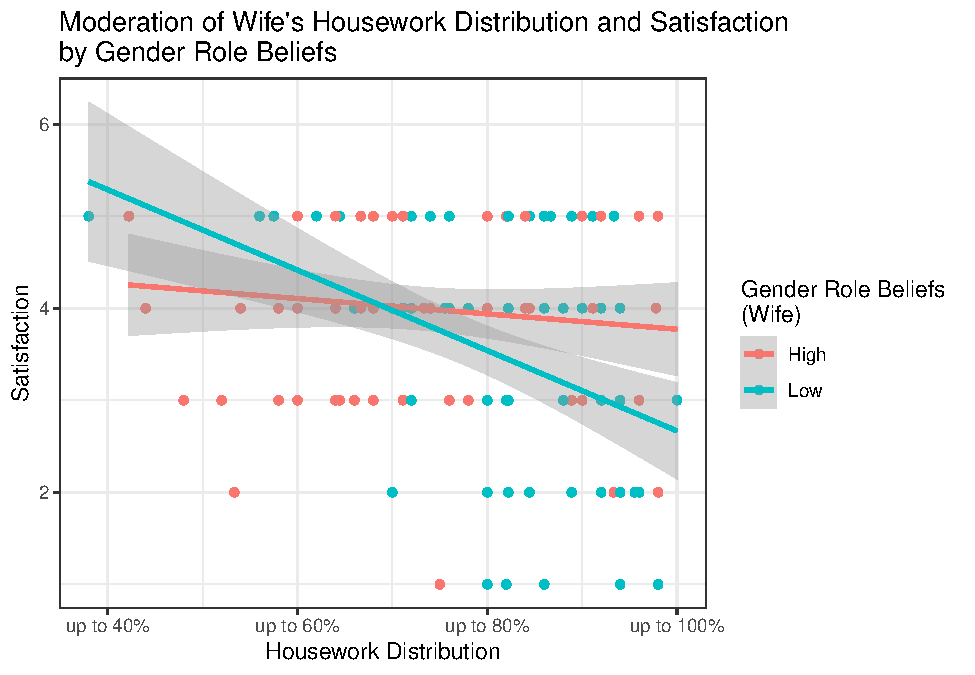
\includegraphics{results_files/figure-latex/unnamed-chunk-14-1.pdf}
\caption{\label{fig:unnamed-chunk-14}Moderation of wife's housework distribution and satisfaction by gender role beliefs. Housework distribution in \%, Satisfaction and gender role beliefs were measured with a 5 point Likert scale (1 = liberal, 5 = conservative).}
\end{figure}



Wives who have low gender role beliefs, which means they are more liberal, reported a lower satisfaction with an increasing amount of housework they had to do. Women with more conservative gender role beliefs (high) did not show a significant decrease in satisfaction with an increasing amount of housework (figure 3).

\begin{figure}
\centering
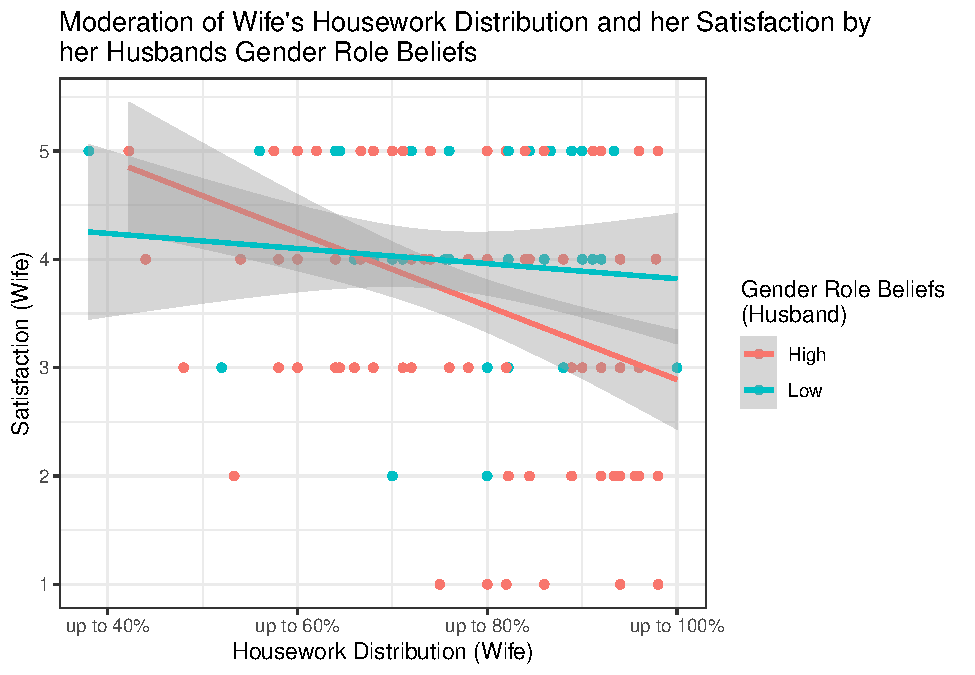
\includegraphics{results_files/figure-latex/unnamed-chunk-16-1.pdf}
\caption{\label{fig:unnamed-chunk-16}Moderation of wife's housework distribution and her satisfaction by their husbands gender role beliefs. Housework distribution in \%, Satisfaction and gender role beliefs were measured with a 5 point Likert scale (1 = liberal, 5 = conservative).}
\end{figure}

As the housework distribution increases for wives whose husbands have low gender role beliefs, their satisfaction remains constant. As the housework distribution increases for wives whose husbands have high gender role beliefs, their satisfaction decreases (figure 4).

\hypertarget{religion}{%
\paragraph{Religion}\label{religion}}

The two intercept model gives us the two coefficients for men and women.

None of the interactions between actors housework distribution and their religion was significantly different for husbands or wives. (\emph{p}\textgreater=0.19,\emph{se}=0.08). None of the results illustrate that the average female-typed tasks completed by the actor or partner from the husband and wife's perspective was related to their religion.

\hypertarget{exploratory-results}{%
\subsection{Exploratory Results}\label{exploratory-results}}

Mediation is a way for researchers to explain the process of one variable affecting another variable. It is essentially a possible explanation for the relationship between the two variables. Mediation assesses whether the effects of the X variable (the independent variable) are significant on the Y variable (the dependent variable), through a third variable called M (the mediator).

Based on our primary analysis so far, we are interested in further exploring how to concept of gatekeeping fits into our research. We want to explore whether gatekeeping is a mediator variable in our relationship between the partners' gender role beliefs and housework tasks. Are women with higher gender role beliefs more likely to gatekeep housework tasks?

The summary table above shows us that all paths are statistically significant (\emph{p}\textless=0.00). Not all the paths are positive, the effect of the partner gender role beliefs on the actor's satisfaction is negative. So, the partner's gender role beliefs could negatively impact the actor's satisfaction. The effect of the actor's gender role beliefs on the actor's satisfaction is 0.52 which means that the actor's gender role beliefs could positively impact the actor's satisfaction.

The summary table above shows us that not all paths are statistically significant. The effect of the actor's gender role beliefs on the actor's gatekeeping behaviors could be potentially mediated (\emph{p} =0.00). This path is also positive, so the actor's gender role beliefs could positively impact the actor's gatekeeping behaviors.

I DONT UNDERSTAND WHAT A B PATH IS SO I CANT ADD MY ANALYSIS THIS THIS PART - DO EITHER OF YOU UNDERSTAND IT?(a path, the effect the explanatory variable has on the mediator, c path: the effect the explanatory had on the response. B path: the effect the mediator has on the response while controling for the explanatory variable. c` means the effect the explanatory variable has on the predictor after controling for the mediator. To find how much effect the mediator has, we do ab/c*100 )(in context of our study b path means the effect of gatekeeping on satisfaction while controlling for housework distribution.If b paths are significant but none of the a paths, then we found a partial mediation)

\hypertarget{sobel-test}{%
\paragraph{Sobel Test}\label{sobel-test}}

The Sobel test measures whether gatekeeping influences how the female partner's gender role beliefs affects her satisfaction. Looking at the p-value from results table above, the data are not statistic. Gatekeeping doesn't have a significant influence on this relationship.

\hypertarget{references}{%
\section{References}\label{references}}

\hypertarget{refs}{}
\begin{CSLReferences}{1}{0}
\leavevmode\vadjust pre{\hypertarget{ref-kenny2020dyadic}{}}%
Kenny, D. A., Kashy, D. A., \& Cook, W. L. (2020). \emph{Dyadic data analysis}. Guilford Publications.

\end{CSLReferences}


\clearpage
\renewcommand{\listfigurename}{Figure captions}

\clearpage
\renewcommand{\listtablename}{Table captions}


\end{document}
